\documentclass[8pt]{article}
\usepackage[a4paper,landscape,margin=1in]{geometry}
\usepackage{cmbright}

\usepackage{amsmath}
\usepackage{nicefrac}
\usepackage{siunitx}

\usepackage{array}
\usepackage{booktabs}
\usepackage{longtable}

\usepackage{xcolor}
\definecolor{urlblue}{HTML}{0000ee}
\usepackage{hyperref}
\hypersetup{%
colorlinks = true,%
urlcolor   = urlblue,%
}

\usepackage{tcolorbox}
\usepackage{varwidth}

\setlength\parindent{0pt}
\pagenumbering{gobble}

\begin{document}
\begin{figure}[!ht]
% MF group logo
\begin{minipage}[b][2.5cm][c]{.72\textwidth}
\href{http://foroozandeh.chem.ox.ac.uk/home}%
{\includegraphics[scale=1.8]{/home/simon/Documents/DPhil/projects/spectral_estimation/NMR-EsPy/nmrespy/images/mf_logo.png}}
\end{minipage}
% NMR-EsPy logo
\begin{minipage}[b][2.5cm][c]{.27\textwidth}
\href{https://foroozandehgroup.github.io/NMR-EsPy}%
{\includegraphics[scale=0.5]{/home/simon/Documents/DPhil/projects/spectral_estimation/NMR-EsPy/nmrespy/images/nmrespy_full.png}}
\end{minipage}
\end{figure}

\texttt{15:11:02\\02-10-2021}

% user provided description
\subsection*{Description}
Gramicidin \textsuperscript{1}H data, region: 4.92 - 4.63Hz. MPM result.

% experiment parameters
\subsection*{Experiment Information}
\hspace{-6pt}
\begin{longtable}[l]{c c}
\toprule
Parameter & F1
\\\midrule
Transmitter frequency (MHz) & 699.85349925\\
Sweep width (Hz) & 213.3550492785903\\
Sweep width (ppm) & 0.30485673002597374\\
Transmitter offset (Hz) & 3341.8042558034504\\
Transmitter offset (ppm) & 4.775005425256435\\
\bottomrule
\end{longtable}

% estimation result
\subsection*{Result}
\begin{longtable}[l]{c c c c c c c c}
\toprule
$m$ & $a_m$ & $\phi_m\ (\text{rad})$ & $f_m\ (\text{Hz})$ & $f_m\ (\text{ppm})$ & $\eta_m\ (\text{s}^{-1})$ & $\int$ & $\nicefrac{\int}{\left\lVert\int\right\rVert}$
\\\midrule
1 & 0.62488 & 1.5269 & \num{3.2557e+3} & 4.652 & 17.83 & 418.41 & \num{4.0626e-3}\\
2 & 0.36299 & 1.0592 & \num{3.2638e+3} & 4.6635 & 9.1135 & 278.19 & \num{2.7012e-3}\\
3 & 0.19188 & \num{-4.8273e-2} & \num{3.274e+3} & 4.6781 & 6.321 & 127.15 & \num{1.2346e-3}\\
4 & 3.1341 & \num{-1.0498e-2} & \num{3.2871e+3} & 4.6968 & 14.628 & \num{2.0792e+3} & \num{2.0189e-2}\\
5 & 6.8836 & 0.24914 & \num{3.2934e+3} & 4.7058 & 18.405 & \num{4.4267e+3} & \num{4.2982e-2}\\
6 & 2.8654 & 0.71841 & \num{3.2956e+3} & 4.7089 & 10.492 & \num{1.9474e+3} & \num{1.8909e-2}\\
7 & 5.9813 & 0.61039 & \num{3.3015e+3} & 4.7175 & 15.041 & \num{3.7191e+3} & \num{3.6112e-2}\\
8 & 0.66861 & 0.44685 & \num{3.3048e+3} & 4.7221 & 8.479 & 434.39 & \num{4.2178e-3}\\
9 & 1.6055 & 0.53928 & \num{3.3104e+3} & 4.7301 & 9.9977 & \num{1.0462e+3} & \num{1.0159e-2}\\
10 & 5.3108 & 0.46259 & \num{3.3203e+3} & 4.7442 & 19.976 & \num{3.1777e+3} & \num{3.0855e-2}\\
11 & 37.022 & 0.25519 & \num{3.3217e+3} & 4.7463 & 11.471 & \num{2.377e+4} & 0.2308\\
12 & 36.964 & 0.15068 & \num{3.3275e+3} & 4.7546 & 12.726 & \num{2.4248e+4} & 0.23544\\
13 & 95.138 & 0.1537 & \num{3.3306e+3} & 4.759 & 14.607 & \num{6.238e+4} & 0.60569\\
14 & 80.67 & 0.31912 & \num{3.3363e+3} & 4.7672 & 13.391 & \num{5.0822e+4} & 0.49347\\
15 & 32.753 & \num{6.3159e-2} & \num{3.3396e+3} & 4.7718 & 12.096 & \num{2.1688e+4} & 0.21059\\
16 & 31.236 & 0.18062 & \num{3.3454e+3} & 4.7802 & 10.584 & \num{2.0388e+4} & 0.19796\\
17 & 100.61 & -0.96059 & \num{3.3465e+3} & 4.7817 & 66.005 & \num{4.3835e+4} & 0.42562\\
18 & 8.6332 & \num{6.9032e-3} & \num{3.351e+3} & 4.7882 & 18.599 & \num{5.7278e+3} & \num{5.5615e-2}\\
19 & 13.288 & 0.27247 & \num{3.3581e+3} & 4.7983 & 22.636 & \num{8.4908e+3} & \num{8.2444e-2}\\
20 & 2.3573 & 0.73585 & \num{3.3655e+3} & 4.8088 & 17.314 & \num{1.4562e+3} & \num{1.414e-2}\\
21 & \num{6.2193e-2} & -0.32478 & \num{3.3759e+3} & 4.8237 & 4.1461 & 41.637 & \num{4.0428e-4}\\
22 & 5.4058 & 0.58703 & \num{3.4015e+3} & 4.8604 & 74.472 & \num{2.9837e+3} & \num{2.8971e-2}\\
23 & 0.12143 & -1.7837 & \num{3.4069e+3} & 4.868 & 5.6225 & 109.64 & \num{1.0646e-3}\\
24 & \num{2.7522e-2} & 1.5426 & \num{3.4185e+3} & 4.8846 & 2.4326 & 30.203 & \num{2.9326e-4}\\
25 & 2.7069 & 2.9526 & \num{3.4345e+3} & 4.9074 & 75.653 & \num{1.7615e+3} & \num{1.7103e-2}\\
\bottomrule
\end{longtable}

% figure of result
\begin{center}
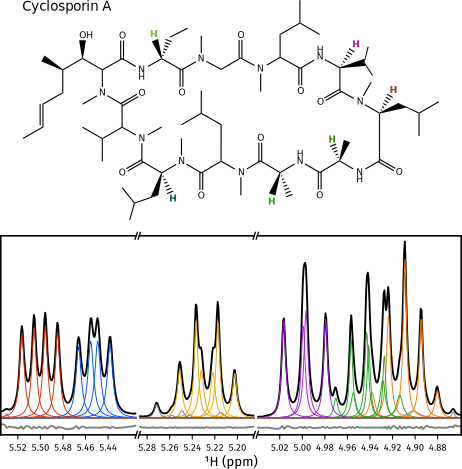
\includegraphics{/tmp/figure.pdf}
\end{center}

% blurb
\small
\begin{tcolorbox}[hbox]
\begin{varwidth}{\textwidth}
Estimation performed using \textsc{NMR-EsPy}.\\
Author: Simon Hulse\\
For more information:\\[5pt]
{\raisebox{-4pt}{\includegraphics[scale=0.029]{/home/simon/Documents/DPhil/projects/spectral_estimation/NMR-EsPy/nmrespy/images/book_icon.png}}}\hspace{1em}\href{https://foroozandehgroup.github.io/NMR-EsPy}{\texttt{https://foroozandehgroup.github.io/NMR-EsPy}}\\[5pt]
{\raisebox{-4pt}{\includegraphics[scale=0.12]{/home/simon/Documents/DPhil/projects/spectral_estimation/NMR-EsPy/nmrespy/images/github.png}}}\hspace{1em}\href{https://github.com/foroozandehgroup/NMR-EsPy}{\texttt{https://github.com/foroozandehgroup/NMR-EsPy}}\\[5pt]
{\raisebox{-3pt}{\includegraphics[scale=0.015]{/home/simon/Documents/DPhil/projects/spectral_estimation/NMR-EsPy/nmrespy/images/email_icon.png}}}\hspace{1em}\href{mailto:simon.hulse@chem.ox.ac.uk?subject=NMR-EsPy query}{\texttt{simon.hulse@chem.ox.ac.uk}}\\[5pt]
If used in a publication, please cite:\\
\textit{No references yet...}
\end{varwidth}
\end{tcolorbox}

\end{document}
